\documentclass[a4paper, 11pt]{article}
\usepackage[utf8]{inputenc}
\usepackage[T1]{fontenc}
\usepackage[french]{babel}
\usepackage{hyperref}
\usepackage{graphicx,float}
\usepackage{minted}

\hypersetup{colorlinks,linkcolor=black,urlcolor=blue}

\begin{document}

\title{IA1 : Système Expert}
\author{Théo Dézé \and Charles Mallet}
\date{9 Novembre 2018} 

\maketitle

\tableofcontents

\pagebreak

\part{Introduction}

Pour le projet nous avons décider de travailliez sur un problème de diagnostique médical. Nous avons défini différentes maladies qui sont a vrais si le patient les a.

\section{Faits}

Nos faits sont de trois nature soit ce sont des informations sur les symptômes du patient, soit sur ces attributs ou sur les maladies qu'il a. 

Comme nous somme sur un moteur d'inférence 0+ nos faits peuvent valoir une valeur booléenne, une chaîne de caractère ou un chiffre (pas dans ce cas mais on a peut le tester dans cas météorologie\footnote{Disponible dans le répertoire docs du projets.}).

\paragraph{Exemple}

\begin{description}
    \item[Symptômes] La zone des douleurs (Poitrine, Gorge, Abdomen, Aucun), si le patient a de la fièvre, toux et vomissement.
    \item[Attributs] Le sexe de la personne.
    \item[Maladies] Maladie que le patient peut avoir (Rhume, Infarctus, Appendicite, etc).
\end{description}

\section{Règles}

Nous avons organisez notre choix des règles selon un arbre décisionnelle voir figure \ref{arbre}. Cela correspond a des questions que pourrais poser un médecin a un patient pour déterminer la maladie du patient.

il est possibles que le patient est plusieurs maladie possible, cela est dus que notre arbre est très simplifier et que comme nous n'avons pas implémenter le chaînage mixte.

Ce qui oblige l'utilisateur à fournir tous les informations alors que si on avais un chaînage mixte on demanderais au patient que ce qui est utile. 

\begin{figure}[H]
    \centering
    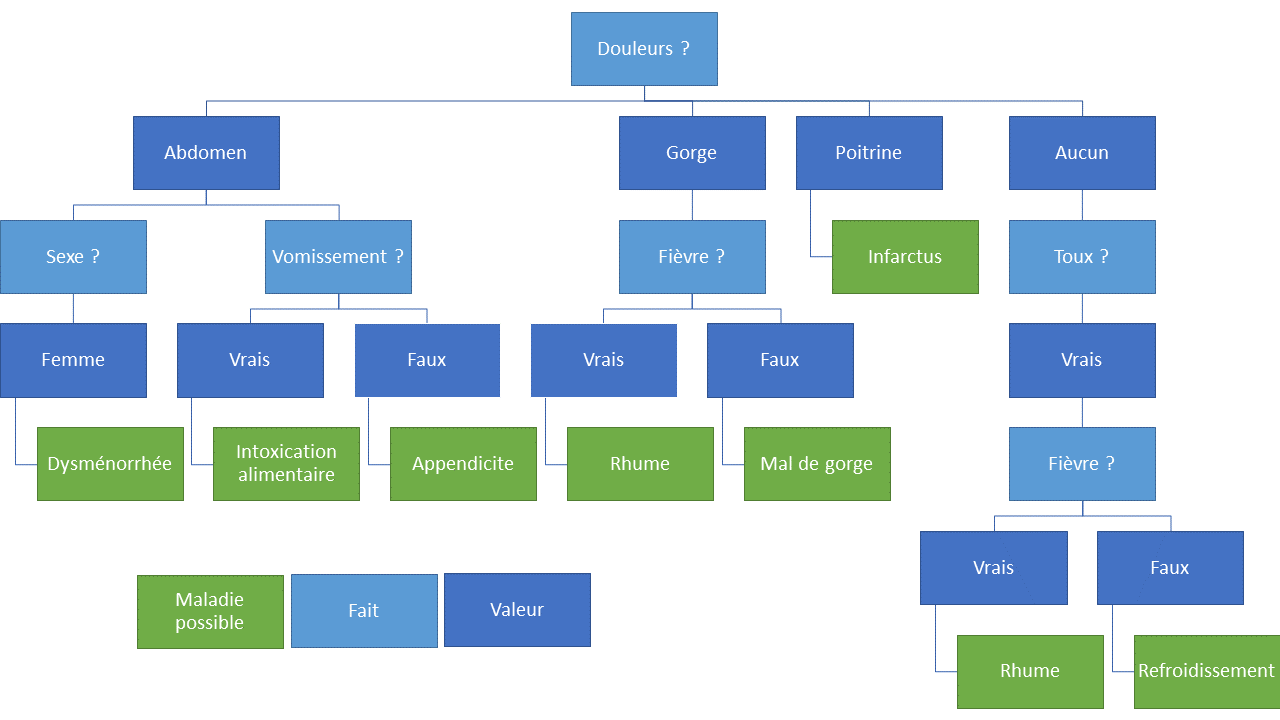
\includegraphics[width=15cm]{arbre.png}
    \caption{\label{arbre} Arbre décisionnelle}
\end{figure}

\section{Choix du langage}

Nous avons choisi de partir sur du python car il présente l'avantage d'être fortement typé mais être dynamique ce qui nous permet facilement de géré les valeurs qui sont de nature différentes.

Pour l'interface on a choisi d'utiliser le package pyside2 qui permet d'utiliser du qt que nous avons déjà vus en C++ avec python et qui est le package officiel.

\part{Système Expert}

\section{Base de connaissance}

Notre base de connaissance est constituer de la base de faits et la base de règles qui sont simplement des tableaux de faits et de règles.

Elle peut être enrichie a l'aide de fichier ou simplement de l'interface.

\subsection{Fichier}

Le fichier permet de déclarer des faits et des règles voir en-dessous.
On ne peut avoir que un fait ou règle par ligne mais on faire une ligne de commentaire avec le symbole '\#'.

Proposition on peut aussi ajouter des ou '||' et des parenthèses, les parenthèses nous on poser un problème ce qui nous a obliger a convertir nos expression in-fixe en post-fixe pour pourvoir les calculer.  

\inputminted{sql}{../maladies.txt}

\subsection{Interface}

Selon l'interface plusieurs méthode sont disponible mais le plus simple qui marche sur les deux est de taper un ligne comme vous le feriez dans le fichier et de validé.

\section{Moteur d'inférence}

Nous avons implémenter le chaînage avant avec but ou juste pour sature la base de connaissance et le chaînage arrière.

A la fin de l'exécution, il affiche un résultat et le cheminement selon la configuration (changeable). Il est possible de voir le log en tapent la commande "log" pour voir tous le commandes disponible, il suffit de taper "aide".

\section{Interface utilisateur}

Nous avons développez deux interfaces, une en ligne de commande et une graphique. 

\subsection{Ligne de commande}

\begin{figure}[H]
    \centering
    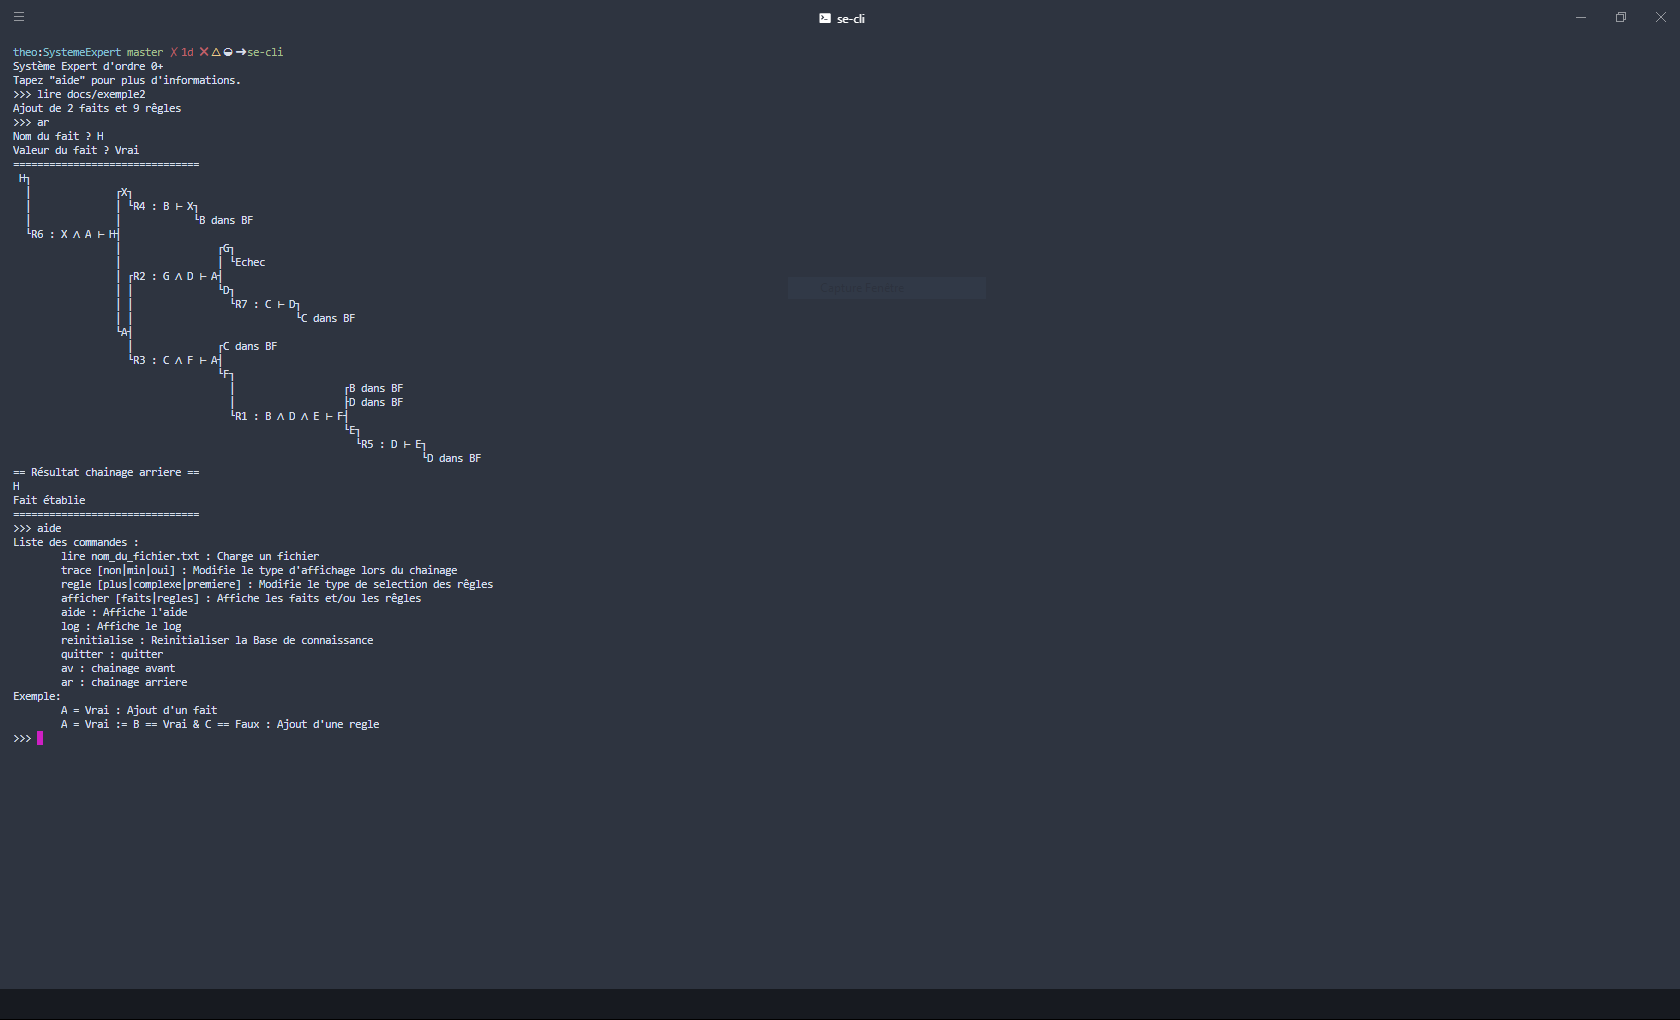
\includegraphics[width=12cm]{cli.png}
    \caption{\label{cli} SE-CLI}
\end{figure}

L'interface un ligne de commande s'inspire de l'interpréteur de python.

\subsection{Graphique}

\begin{figure}[H]
    \centering
    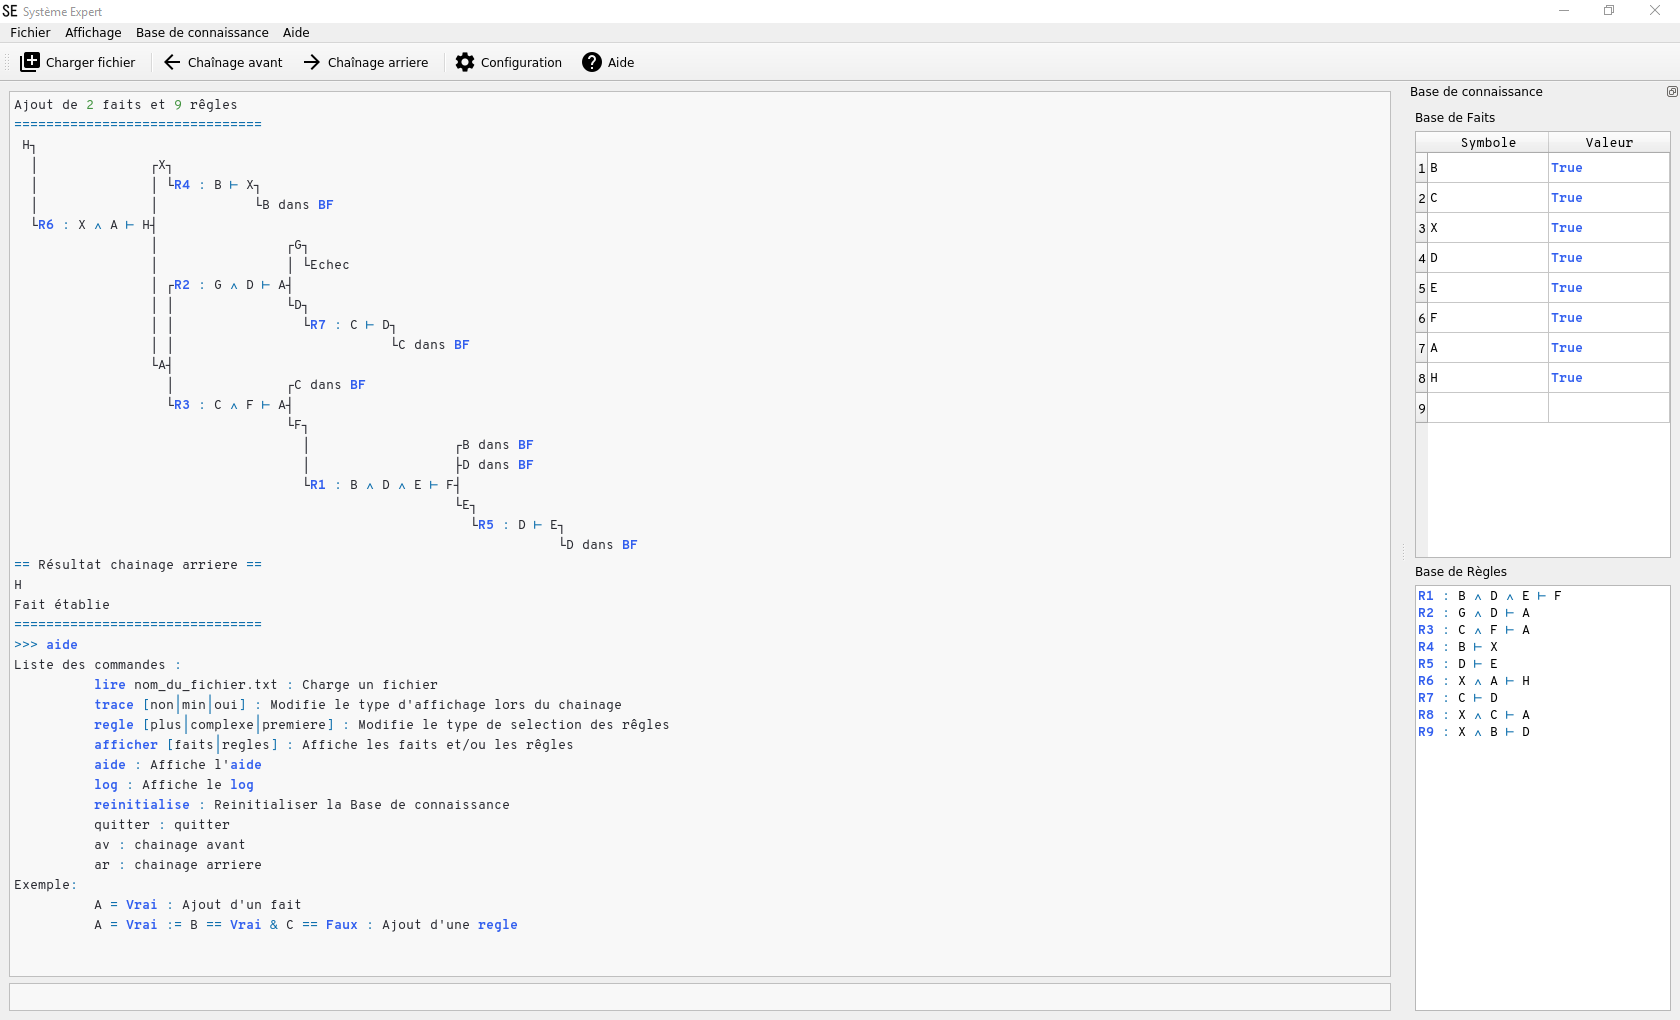
\includegraphics[width=12cm]{gui.png}
    \caption{\label{gui} SE-GUI}
\end{figure}

L'interface permet de simplifier l'utilisation pour un utilisateur qui n'est pas habitué par l'utilisation du terminal.

La plupart des commandes peuvent êtres exécuter à l'aide de bouton. Mais il est toujours possible de taper les commande comme sur la version en ligne de commande.

\paragraph{Composition de l'interface}

\begin{description}
    \item[Terminal] Il est constitué d'un affichage et d'une ligne de saisie. Il s'utilise exactement comme la version en ligne de commande.
    \item[Dock] Il permet d'afficher le base de connaissance et permet de modifier/ajouter un fait très simplement.
    \item[Barre d'outils] Il donne accès aux commandes importantes.
\end{description}

\part{Conclusion}

\section{Améliorations possibles}

Voici une liste des améliorations possibles:

\begin{itemize}
    \item Ajouter des coefficients de certitude. Pour représenter des événements incertains.
    \item Représenter les faits sous la forme de n-uplet pour faciliter les regroupement des faits exemple AgeBob = 25 devient (Bob,age,25) ou ParentsBob = "Léo Léa" devient (Bob,parents,Léo,Léa).
    \item Transformer le moteur 0+ en 1.
\end{itemize}

\section{Le code source du projet}

Tous les code sources du projet et ce document sont disponible sur \url{https://github.com/theodeze/SystemeExpert}

\end{document}